%\subsection{Constraining uncertainty at the Byrd ice core}
\section{Comparing Byrd and WAIS Divide ice core chronologies}\label{byrdwdcompare}
We leverage the assumed relative accuracy of the WAIS Divide ice core chronology to validate our computed age-depth profile at the Byrd ice core. Seven radar layers have been traced between the WAIS Divide and Byrd ice cores using seismic interpretation software, \textit{Landmark} \citep{}. We assume these layers are isochronous \citep{} and so each ice core chronology should estimate them to be the same age to within uncertainty. 



%\subsection{Comparing radar age at Byrd and WAIS Divide ice cores}

%Additional error in the Byrd ice core profile we calculated could be attributed to use of an oversimplified ice flow model. Errors from these sources are assumed independent of errors in the volcanic record or our choice of ice flow parameters and are therefore included in our uncertainty estimates using a root mean square method. 

%\begin{figure}
%%\begin{center}
%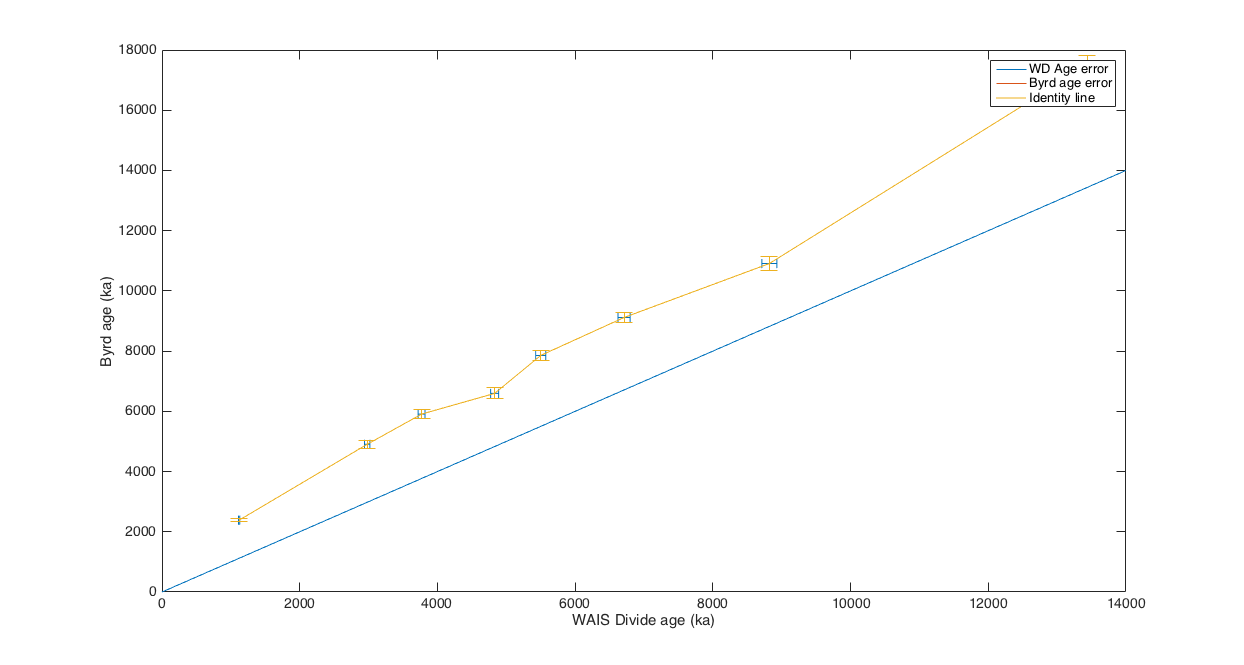
\includegraphics[scale=0.4]{figures/wd-byrd-compare}
%%\captionsetup{width=.9\textwidth}
%\caption[]{Comparison between WAIS Divide and Byrd ages for the 8 layers that can be tracked between them. These values are expected to fall on the identity line to within their error bars, however WAIS Divide ages are consistently higher than Byrd ages for the same layers. This draws into question the Byrd ice core ages, the layers traced between the cores, and the estimate of uncertainty in the Byrd chronology. }
%%\end{center}
%\label{fig:layer_agedepth}
%\end{figure}

%\textbf{This result shows some serious issues with the Byrd chronology. Because the flow model follows the observed volcanic ages so well, this is likely less a flow model thing and more an uncertainty thing. The envelope on uncertainty needs to be much wider. This could be because of large issues with the measurement of depth. Adding the isotope chronology as data may also help with this, which is already in progress for the accumulation inversion. The other thing to check is the tracing of the layers (also in progress by interns), but it's doubtful this would lead to such a systematic problem.}

%Disagreement in the age of a layer outside the assumed uncertainty indicates an underestimation of uncertainty in our previous methods. We assume discrepancies can be attributed to uncertainties in the derived Byrd ice core age-depth profile we computed, rather than the WAIS Divide chronology with its well-constrained uncertainty analysis.